\newpage
\section{Kinematik}

Beschreibt Bewegungen von Massenpunkten und 
Körpern, ohne dabei nach den wirkenden Kräften zu 
fragen.
Ein Körper kann sich auf zwei Arten bewegen: \\
- Translation: Der Körper wird verschoben \\
-  Rotation: Der Körper wird gedreht

\begin{multicols}{2}
\textbf{Geschwindigkeit} \\
Geschwindigkeit entspricht der pro Zeiteinheit \\
zurückgelegte Wegstrecke.  $v:= [m/s]$ \\
Geschwindigkeit: $v = \frac{x_{2} - x_{1}}{t_{2} - t_{1}} = \frac{\Delta s}{\Delta t}$  \\
Mittlere Geschwindigkeit: $ \bar{v} = \frac{x(t + \Delta t) - x(t)}{\Delta t}$  $v = \lim_{t \rightarrow 0} \frac{\Delta x}{\Delta t}$ \\
\columnbreak
\\
\textbf{Beschleunigung} \\
Die Beschleunigung entspricht der Änderung der \\
Geschwindigkeit pro Zeiteinheit. \\
Mittlere Beschleunigung: $\bar{a} = \frac{\Delta v}{ \Delta t} $   \\
$a:= [m/s^2]$ \\
\end{multicols}

\subsection{Bewegungen}
\textbf{Tipp:} Immer in $\frac{m}{s}$ rechnen (d.h. $\frac{Wert \; in \; km}{3.6}$, 	Bremsen: $\alpha < 0$ !)
\begin{multicols}{3}
	\subsubsection{Gleichförmige B.}
	Konstante Geschwindigkeit: \\
	Reibungskraft entspricht der \\
	Motorenleistung. \\
	$a = 0$ \\
	$v = konstant$\\
	$s = vt + s_0$ \\
	\\
	\\
	\adjustbox{width=5cm}{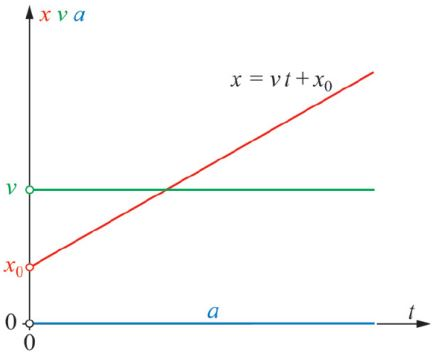
\includegraphics{bilder/gleichfBeschl}}
\columnbreak
	\subsubsection{Gleichmässig beschl. B.}
	$a = konstant$ \\
	$v = \alpha t + v_{0} = \dot s = s'(t)$ \\
	$s = \frac{a}{2}t^2 + v_{0}t + s_{0} = \frac{v_{1}^2 - v_{0}^2}{2a}$ \\
	$a = \frac{v_{1}^2 - v_{0}^2}{2s} = \frac{\Delta v}{\Delta t} = \dot v = s''(t)$ \\
	$v_{2} = \sqrt{v_{0}^2 + 2as}$ \\
	\\
	\\
	\adjustbox{width=5cm}{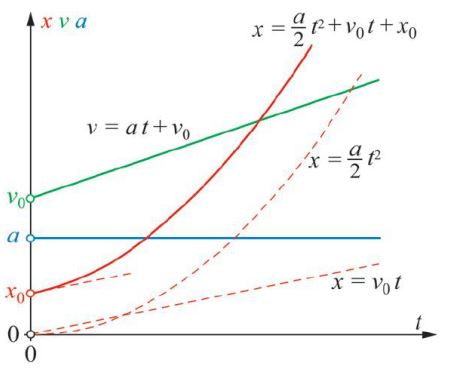
\includegraphics{bilder/gleichmBeschl}}
\columnbreak
	\subsubsection{Benötigte Werte}
	$s_{0}$ = Anfangsstrecke \\
	$v_{0}$ = Startgeschwindigkeit \\
	$v_{1}$ = Endgeschwindigkeit \\
	$\alpha$ = Winkelbeschleunigung $\; [\frac{rad}{s^2}]$ \\
	$\omega:$ = Winkelgeschwindigkeit $\; [\frac{rad}{s}]$ \\
	$\varphi$ = Winkel $\; [rad]$ \\
	$T$ = Periode \\
	$f$ = Frequenz \\
	$\omega_{0}$ = Startwinkelgeschwindigkeit  \\
	$\omega_{1}$ = Endwinkelgeschwindigkeit  \\
	$\varphi_{0}$ = Startwinkel  \\
	$a_{z}$ = Zentralbeschleunigung \\
	$n$ = Drehzahl = Umdrehungen pro Zeiteinheit\\
	\\
	$ \omega = 2 \pi n = 2 \pi f$ \\
	$ n = f = \frac{1}{T} = \frac{1}{\frac{2 \pi}{\omega_0}} = \frac{\omega_o}{2\pi}$
\end{multicols}
	
\subsection{Kreisbewegung}
RADIANT und nicht Grad verwenden! |
Umrechung DEG $\overrightarrow{}$ RAD: $\cdot \frac{2\pi}{360}$ | 
Umrechnung RAD$\overrightarrow{}$ DEG: $\cdot \frac{360}{2\pi}$
\begin{multicols}{3}
	\subsubsection{Gleichf"ormige}
	$a = 0 \\
	s = r\varphi \\
	v = r\omega \\
	\omega = \dot \varphi = \frac{v}{r} = 2\pi f\\
	\varphi = \omega t \\
	f = \frac{1}{T} \\
	\overrightarrow{v} = \overrightarrow{\omega} \times \overrightarrow{r}$ \\
	\\
	\\
	\\
	\columnbreak
\subsubsection{Gleichf"ormig beschl.}
	$\alpha = konstant = \dot \omega = \varphi''(t) \\
	a = r \alpha \\
	\omega = \alpha t + \omega_{0} = \sqrt{\omega_{0}^2 + 2 \alpha(\varphi - \varphi_{0})}$ \\
	$\varphi =\frac{a}{2}t^2 + \omega_{0}t + \phi_{0} = \frac{\omega_{1}^2 -\omega_{0}^2}{2a}$	\\
	\adjustbox{width=2.5cm}{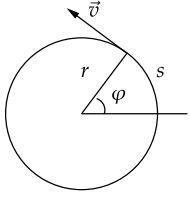
\includegraphics{bilder/gleichfKreis_k}}
	\columnbreak
	\subsubsection{Zentripetalbeschleunigung}
	$\alpha_{z} = \frac{v^2}{r} = r\omega^2 \\
	v = \frac{2\pi r}{T} \\
	F_{z} = ma_{z} = \frac{mv^2}{r} = m\omega^2r$ \\
	\\
	\adjustbox{width=2.5cm}{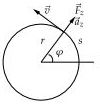
\includegraphics{bilder/zentripetal_k}}
\end{multicols}

\newpage
	\subsection{Wurfbahnen}
	
	\begin{multicols}{3}
		\textbf{Freier Fall} \\
		$a_{y} = -g \\
		v_{y} = -gt \\
		h(t) = y(t) = -\frac{g}{2}t^2 \\
		v_{max} = \sqrt{2gh_0} \\
		t_{max} = \sqrt{\frac{2h_0}{g}}$ \\
		\\
		\\
		\\
		\adjustbox{width=1cm}{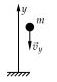
\includegraphics{bilder/hwurf_k}}
	
		\columnbreak
		\textbf{Senkrechter Wurf $\uparrow$} \\
		Gleichmäsig beschl.: $a = -g$ \\
		Steigzeit: $t_{s} = t_{max} = \lvert{\frac{v_{0}}{g}}\rvert$ \\
		Flugzeit: $t_{f} = 2t_{s}$ \\
		$y(t) = -\frac{g}{2}t^2 + v_0 t, $\\
		$v(t) = -gt + v_0$ \\
		Max. Steighöhe: $h_{max} = \frac{v_{0}t}{2} = \lvert{\frac{v_{0}^2}{2g}}\rvert$ \\
%		\adjustbox{width=1cm}{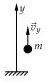
\includegraphics{bilder/hwurf_k3}}

		\textbf{Senkrechter Wurf $\downarrow$} \\
	
		$y(t) = y_0 - v_0t - \frac{g}{2}t^2$ \\
		$v(t) = -gt - v_0$ \\
		Fallzeit: $t_{max} = \frac{-v_{0} + \sqrt{v_0^2 + 2g + y_0}}{g}$ \\

		
	
		\columnbreak
		\textbf{Horizontaler Wurf} \\
		$a_{x} = 0 \rightarrow{} v_{x} = v_{0}$  \\
		$a_{y} = -g \rightarrow{} v_{y} = -gt$ \\
		$y(t) = s_{y} = -\frac{g}{2}t^2 = -\frac{g}{2v_{0}^2}s_{x}^2$ \\
		Flugzeit: $t_{max} = \sqrt{\frac{s \cdot h}{g}}$ \\
		Flugstrecke: $s_{x} = vo \cdot t_{max} = v_0 \sqrt{\frac{2y_0}{g}}$ \\
		$v_{Ges} = \sqrt{v_{x}^2 + v_{y}^2} $ \\
		Parabelgleichung:\\
		\adjustbox{width=2.5cm}{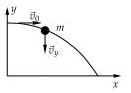
\includegraphics{bilder/hwurf_k2}}
	\end{multicols}
	
	\subsubsection{Schiefer Wurf}
\begin{multicols}{3}
	Gleichförmig in x-Richtung \\
	$a_{x} = 0$ \\
	$v_{x} = v_{0x} = v_0 \cdot \cos(\varphi)$ \\
	$v(t)= v_{0x} \cdot t $\\
	\\
	\adjustbox{width=2.5cm}{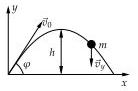
\includegraphics{bilder/schief_k}}
\columnbreak
	\\
	Gleichmässig in y-Richtung \\
	$a_{y} = -g$ (nimmt immer ab)\\
	$v_{y} = v_{oy} - g \cdot t = v_0 \cdot \sin(\varphi) - g \cdot t $ \\
	$v(t) = -\frac{1}{2} \cdot a \cdot t^2 + v_{0y} \cdot t + 0$ \\
	$d = \frac{v_{0}^2}{g} \cdot \sin{(2\varphi)} \\$
	$h = \frac{v_{0}^2}{2g}\sin^2{\varphi}$ \\
	$t = \frac{2v_{0} \cdot \sin{\varphi}}{g}$ \\
\columnbreak
\\
	$\Delta y = v_{0}\sin{\varphi}t - \frac{gt^2}{2}$ \\
	$\Delta y = v_{0}\cos{\varphi}t$ \\
	Max. Wurfweite: $x_{Wurf} = \frac{\sin2\alpha \cdot v_{0}^2}{g} \overrightarrow{}$ \\ $\sin2\alpha = 1 \; \overrightarrow{} \alpha = 45^\circ$ \\
	Spez. Wurfweite: $\alpha < 45^\circ \; (Flachwurf)$ \\
	$ \alpha > 45^\circ$ \; (Steilwurf)\\
	Max. H"ohe: Halbe Wurfweite \\
\	Parabelgleichung: $y = \tan{\varphi}s_{x} - \frac{gs_{x}^2}{sv_{0}^2cos^2{\varphi}}$ \\
%	$ y = \frac{1}{2} g \frac{x^2}{v_{0x}^2} + v_{oy} \frac{x}{v_{0x}$\\
\end{multicols}

\subsubsection{Analogie Translation und Rotation}
\begin{tabular}{|l|l|l|l|l|l|}
	Symb & Grösse 			& Beziehung 									& Symb. 		& Grösse 					& Beziehung \\
	$s$  & Weg 				& 												& $\varphi$ 	& Winkel 					& \\
	$v$  & Geschwindigkeit 	& $v = \frac{ds}{dt}$ 							& $\omega$ 		& Winkelgeschwindigkeit 	& $\omega = \frac{d\varphi}{dt}$ \\
	$a$  & Beschleunigung 	& $a = \frac{dv}{dt}$ 							& $\alpha$ 		& Winkelbeschleunigung 		& $\alpha = \frac{d\omega}{dt}$ \\
	$m$  & Masse 			& 												& $J$ 			& Trägheitsmoment 			& $J = \int r^2 dm$ \\
	$p$  & Impuls 			& $p = mv$ 										& $L$ 			& Drehimpuls 				& $L = J\omega$ \\
	$F$  & Kraft 			& $F = \frac{dp}{dt}$ 							& $M$ 			& Drehmoment 				& $M = \frac{dL}{dt}$ \\
	$dW$ & Arbeit 			& $dW = \overrightarrow{F}\overrightarrow{ds}$ 	& $dW$ 			& Arbeit 					& $dw = Md\varphi$ \\
	$P$  & Leistung 		& $P = \overrightarrow{F}\overrightarrow{v}$ 	& $P$ 			& Leistung 					& $P = M\omega$ \\
	$E_{trans}$ & Translationsenergie & $E_{trans} = \frac{mv^2}{2}$ 			& $E_{rot}$ 	& Rotationsenergie 			& $E_{rot} = J\omega^2 2$ \\
	
\end{tabular}					

%\adjustbox{width=12cm}{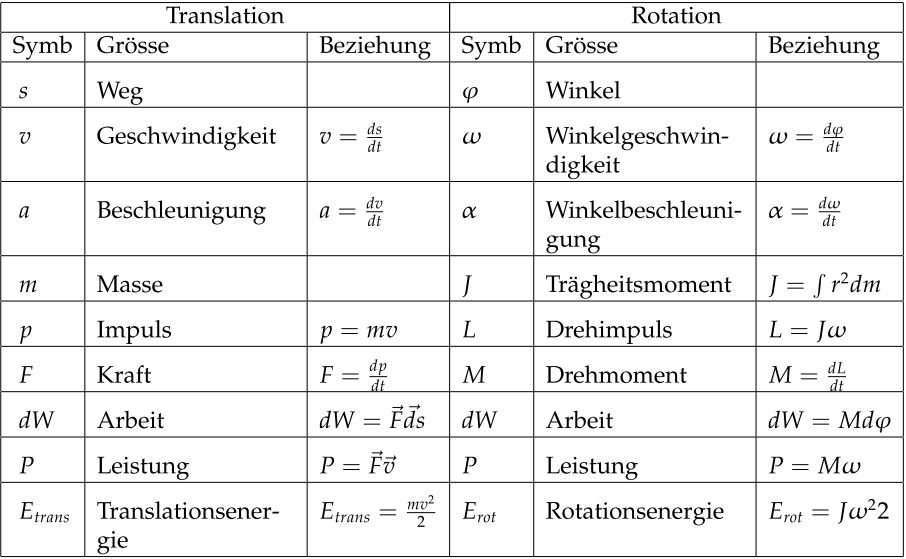
\includegraphics{bilder/trans-rotation}}